\documentclass[draftclsnofoot,onecolumn]{IEEEtran}
\usepackage{url}
\usepackage{listings}  
\usepackage[pdftex]{graphicx}
\usepackage[caption=false,font=footnotesize]{subfig}
\usepackage[section]{placeins}

%Configure graphicx package
\graphicspath{{./images/}}
\DeclareGraphicsExtensions{.jpeg,.png}

% Configure the lstlisting package 
% en.wikibooks.org/wiki/LaTeX/Source_Code_Listings#Using_the_listings_package
\lstdefinestyle{cSharp}{
	language=[Sharp]C, 
	basicstyle=\small\ttfamily, 
	lineskip={-0.1pt},
	tabsize=4,
	aboveskip=15pt,
	belowskip=0pt,
    numbers=left
}
\lstMakeShortInline^

%Improve readability of table of contents
\renewcommand\thesubsection{\Alph{subsection}}

% No IEEEtrans section headers since we want our requrments to have numbers
%\renewcommand\thesection{\arabic{section}}
%\renewcommand\thesubsection{\thesection.\arabic{subsection}}
%\renewcommand\thesubsubsection{\thesubsection.\arabic{subsubsection}}

%\renewcommand\thesectiondis{\arabic{section}}
%\renewcommand\thesubsectiondis{\thesectiondis.\arabic{subsection}}
%\renewcommand\thesubsubsectiondis{\thesubsectiondis.\arabic{subsubsection}}

% Example of Constructing an image figure: (change label to unique identifier)
%\begin{figure}[!htb]
%\centering
%\includegraphics[scale=1]{myfigure}
%\caption{Simulation results for the network.}
%\label{fig_sim}
%\end{figure}

% Example of Constructing a code example figure: (change label to unique 
% identifier)
%\begin{figure}[!htb]
%\centering
%\begin{lstlisting}
%public class Logger
%{
%	public virtual void Log(Log log)
%	{
%		Console.WriteLine(log);
%	}
%	public virtual void LogAll(IEnumerable<Log> logs)
%	{
%		foreach(var l in logs)
%		{
%			Log(l);
%		}
%	}
%}
%\end{lstlisting}
%\caption{Simulation results for the network.}
%\label{fig_sim1}
%\end{figure}

% Exapmle of refering to figure
% Blah, blah, and here is Figure \ref{fig_sim}

\begin{document}
\lstset{style=cSharp}
\title{Semantic Diff via C\# Compiler Platform}
%\IEEEspecialpapernotice{Group 19 Winter 2016 Progress Report}

\author{Shawn Fontaine, Cody Ray Hoeft, Michael Rose\\
	School of Electrical Engineering and Computer Science\\
	Oregon State University
\thanks{Group 19 Winter 2016 Progress Report}
\thanks{Proposer/Client: Philip Carter of Microsoft.}}

\maketitle
\pagenumbering{gobble} %removes page number

\begin{abstract}
Large colaborative software projects involve constantly changing repositories, numerous merge conflicts, and subtle runtime errors caused by semantic conflicts. These issues cause a large investment of time that could be used to work on more meaningful changes to the project. Current merge tools examine differences in the text between versions of code. Without using the semantics of the code results in unnecessary conflicts and subtle bugs being missed. SemDiff is a Roslyn Analyzer for C\# projects that helps identify non-semantic code changes that can be ignored as well as semantic changes that introduce potential runtime errors. SemDiff produces a NuGet package that is installed with Visual Studio. The package provides visual warnings of non-meaningful conflicts and identifies potential locations for runtime errors. Alerting developers early reduces bug counts and time saved for both developers and project managers. Bug counts are lowered by reducing the quantity of subtle bugs caussed by semantic conflicts. Reducing runtime bugs allows developers to spend less time replicating and debugging hard to find runtime errors and less merge conflicts allow developers and managers to use less time resolving merge conflict manually. 
\end{abstract}

\newpage
\setcounter{tocdepth}{2}
\tableofcontents


\newpage
\pagenumbering{arabic}

%-----------------------------------------------------------------------------|
%%%%%%%%%%%%%%%%%%%%%%%%%%%%%%%%%%%%%%%%%%%%%%%%%%%%%%%%%%%%%%%%%%%%%%%%%%%%%%|
\section{Introduction}%%%%%%%%%%%%%%%%%%%%%%%%%%%%%%%%%%%%%%%%%%%%%%%%%%%%%%%%|
%%%%%%%%%%%%%%%%%%%%%%%%%%%%%%%%%%%%%%%%%%%%%%%%%%%%%%%%%%%%%%%%%%%%%%%%%%%%%%|
%-----------------------------------------------------------------------------|

%%%%%%%%%%%%%%%%%%%%%%%%%%%%%%%%%%%%%%%%%%%%%%%%%%%%%%%%%%%%%%%%%%%%%%%%%%%%%%%
\subsection{Overview}%%%%%%%%%%%%%%%%%%%%%%%%%%%%%%%%%%%%%%%%%%%%%%%%%%%%%%%%%%
%%%%%%%%%%%%%%%%%%%%%%%%%%%%%%%%%%%%%%%%%%%%%%%%%%%%%%%%%%%%%%%%%%%%%%%%%%%%%%%

This report details the motivation, purpose, methodology, and results of the `Semantic Diff via C\# Compiler Platform' (SemDiff) project. The introduction contains a background section, explains the motivation and purpose, and the overall progress of the project. Then the project progress section provides a section on each project requirement that contain the overall progress, current and future work, problems encountered, and the solutions to problems when applicable. Throughout the paper, interesting code and images are included to further explore and explain parts of SemDiff. The report's conclusion summarizes the current status of the project and a glossery defines technical terms used throughout the document.

%%%%%%%%%%%%%%%%%%%%%%%%%%%%%%%%%%%%%%%%%%%%%%%%%%%%%%%%%%%%%%%%%%%%%%%%%%%%%%%
\subsection{Background}%%%%%%%%%%%%%%%%%%%%%%%%%%%%%%%%%%%%%%%%%%%%%%%%%%%%%%%%
%%%%%%%%%%%%%%%%%%%%%%%%%%%%%%%%%%%%%%%%%%%%%%%%%%%%%%%%%%%%%%%%%%%%%%%%%%%%%%%

Mass collaboration in large software projects results in considerable 
overhead. Repositories for these projects contain dozens of pull requsts a 
week from numerous contributors. It is difficult for every developer to be 
fully aware of all pending changes to the repository. Conflicting changes to a 
file occurs often and result in merge conflicts. The common workflow is that 
developers will identify issues---bugs or new features. A developer will make 
a branch, change the source to fix the issue, and then create a pull request. 
After creation, the pull request reviewed by peers and management merges the 
changes into the repository.

Git is one of the most popular version control systems. In order to resolve 
conflicts such as the above, git uses a text-based three-way merge. A three-
way merge compares two files while also considering the ancestor of both 
files. If a section of code differs in all three files it is marked as a 
conflict and the user must resolve it manually. The merge is generic and 
allows Git to use the same algorithm for all text files regardless of their 
content.

Two major problems arise since current tools do not consider the meaning of 
the code being compared. The first problem is when a conflict is identified 
but semantically there should be no conflict. This is known as a false-
positive. For example, consider the situation of the ``moved method'' 
conflict. Suppose a developer, Adam, edits a method in a large file to fix a 
big. Adam passes all tests so he creates a pull request with his changes. 
Before the changes are merged, another developer, Bob, moves the location of 
the method that Adam had edited. Bob might be moving the method because he was 
refactoring the code, introducing a new method, or other code maintenance. Bob 
is unaware that Adam edited the method because his development environment 
provides no information about Adam's pull request. Bob's code passes all tests 
so he creates a pull request. Later their manager, Chris, verifies that the 
pull requests have been peer reviewed and attempts to merge them both into the 
repository. One of the pull requests will merge correctly, however the other 
will fail because of a conflict. Semantically there is no conflict between 
Adam's and Bob's changes. The program will run the same whether the method was 
moved or not. However, Chris now must take extra time to manually review and 
resolve the conflict.

The second problem is known as a false-negative. A false-negative occurs when 
text-based tools do not find a conflict between changed files even though 
there is a semantic conflict. False-negatives are subtle and can introduce 
runtime bugs that are difficult to locate. These conflicts usually occur 
across files that have a semantic connection. For example a developer, Ross, 
is implementing a new ^DatabaseLogger^. The project already has a generic 
^Logger^ that writes logs to the console as shown in Figure~\ref{example1}. 
Ross creates a ^DatabaseLogger^ class derived from ^Logger^ and overrides the 
^Log^ method with new logic to store logs in a database. Ross does not override 
^LogAll^ because he sees that it merely delegates to the ^Log^ method. 
However, before Ross' changes are merged in another developer, Smith, notices 
that it is inefficient for the ^Logger^ in Figure~\ref{example1} to be calling 
^Log^ for every log instead of writing them all at once, so Smith creates the 
logger shown in Figure~\ref{example2}. Smith is unaware of Ross' work and Ross 
is unaware of Smith's work. When their manager, Chris, merges their pull 
requests he finds that they merge with out errors. After all, Ross and Smith 
edited different files. Even though they merge without error and both Ross' 
and Smith's versions work correctly there is now a bug in the code. Calling 
the ^LogAll^ method on the ^DatabaseLogger^ will not log to the database but 
to the console. Because of the subtle nature of this bug, it will be difficult 
to debug and may be a long time before it is reported.

\begin{figure}[!htb]
\centering
\begin{lstlisting}
public class Logger
{
    public virtual void Log(Log log)
    {
        Console.WriteLine(log);
    }
    public virtual void LogAll(IEnumerable<Log> logs)
    {
        foreach(var l in logs)
        {
            Log(l);
        }
    }
}
\end{lstlisting}
\caption{Example for illustrating false-positive conflicts. Shows a generic 
logger}
\label{example1}
\end{figure}

\begin{figure}[!htb]
\centering
\begin{lstlisting}
public class Logger
{
    public virtual void Log(Log log)
    {
        Console.WriteLine(log);
    }
    public virtual void LogAll(IEnumerable<Log> logs)
    {
        Console.WriteLine(string.Join(Environment.NewLine, logs));
    }
}
\end{lstlisting}
\caption{Example for illustrating false-positive conflicts. Shows an override 
of the generic logger shown in Figure~\ref{example1}}
\label{example2}
\end{figure}

Both of these problems illustrate the problem with text-based diffs. A large 
amount of time is spent resolving conflicts that should have never occured and 
locating bugs that could have been identified ahead of time. All of this time 
could be used by the project managers to make more meaningful improvements. 
Understanding the semantics of programs create a barrier for making tools that 
can understand false-positives and false-negative. With most languages, 
retriving information about a program's semantics can be challenging. It may 
be necessary to build a parser, define an abstract syntax tree, and build all 
the logic for understanding what the syntax constructs do. All that work is 
redundant because the languages compiler already has the semantic information. 
The compiler is also the best source for semantic information because it 
implements the semantics. Most compilers are black boxes, files go in and 
programs come out. However, the idea of the compiler as a service has become 
more popular. With a compiler as a service model, the compiler provides a 
large API for inspecting and interpreting both the syntax trees and the 
semantic models of the code. 

In 2015, Microsoft released a new C\# and Visual Basic compiler refered to as `
Roslyn' that uses the compiler as a service model. Roslyn provides a rich API 
including a ^SyntaxTree^ object that represents the abstract syntax tree of a 
file, a ^SemanticModel^ object that represents how a single ^SyntaxTree^ is 
connected to others, and a ^DiagnosticAnalyzer^ interface. The ^SyntaxTree^ 
and ^SemanticModel^ both have a powerful interface for querying their data and 
getting the semantic information from the code. This API lowers the bar for 
developers that want to analyze the semantics of their code, this is why 
Roslyn provides the ^DiagnosticAnalyzer^ abstract class. It provides callbacks 
that can be used to implement custom logic that can report ^Diagnostic^ 
messages back to Roslyn. The analyzers are integrated into the Roslyn pipeline 
when installed; ^Diagnostic^ messages from the analyzer are shown alongside 
compiler generated messages. When this analyzer is installed it is integrated 
into the Roslyn pipeline and any ^Diagnostic^ messages are shown alongside 
compiler generated messages. These analyzers are commonly packaged as NuGet 
packages and installed to projects much like other software dependencies can 
be installed. Additionally, analyzers are tied to the project therefore only 
one developer needs to install an analyzer for all the projects developers to 
start receiving diagnostics.

%%%%%%%%%%%%%%%%%%%%%%%%%%%%%%%%%%%%%%%%%%%%%%%%%%%%%%%%%%%%%%%%%%%%%%%%%%%%%%%
\subsection{Project Purpose and Goals}%%%%%%%%%%%%%%%%%%%%%%%%%%%%%%%%%%%%%%%%%
%%%%%%%%%%%%%%%%%%%%%%%%%%%%%%%%%%%%%%%%%%%%%%%%%%%%%%%%%%%%%%%%%%%%%%%%%%%%%%%

The solution to handling the problems of text based diff is to use semantics. 
SemDiff takes the important first step of being able to locate and identify 
the situations that create false-positive and false-negative merge conflicts. 
Both of the narratives in the background section could have been prevented if 
the developer had been warned that someone else was working in an area that 
could cause problems. If Adam had known that Bob had moved the method, he 
might have moved the method in his also. If Bob had known that Adam edited the 
method, he might not have moved it. Similarly, if Ross had known about Smith's 
changes to the ^Logger^, he would have implemented the ^LogAll^ method. This 
tool could be created with the ability to locate false-negatives and false-
positives, fix the conflicts, and automatically merge the resulting changes. 
However, fixing the resulting conflicts in an automated manner represents an 
extremely challenging task and is beyond the scope of this project.

The goal of SemDiff is not resolving merge conflicts, but preventing false-
negatives and false-positives before they happen by warning developers when 
changes are detected that could cause a merge conflict. This preserves the 
benefits of text-based merging without some of the drawbacks. Text-based diffs 
and merges are fast, dependable, and already exist in every major version 
control system. The drawbacks can also be offset by time spent resolving the 
merge conflicts by hand and building comprehensive test suites to detect false-
positives. However, software projects tend to be short on time and developers 
are expensive resources Not enough time is devoted to test suites and managing 
merge conflicts takes up valuable time. Preventing issues with conflicts helps 
developers focus more on code and less on repository management.

%%%%%%%%%%%%%%%%%%%%%%%%%%%%%%%%%%%%%%%%%%%%%%%%%%%%%%%%%%%%%%%%%%%%%%%%%%%%%%%
\subsection{Overall Progress}%%%%%%%%%%%%%%%%%%%%%%%%%%%%%%%%%%%%%%%%%%%%%%%%%%
%%%%%%%%%%%%%%%%%%%%%%%%%%%%%%%%%%%%%%%%%%%%%%%%%%%%%%%%%%%%%%%%%%%%%%%%%%%%%%%

\subsubsection{Fall Term}

Planning for SemDiff was completed between October and December of 2015. The 
team met with Phillip Carter almost every weekend to talk about the project. 
The project was split into four major parts: handling GitHub interaction, 
false-positive detection, false-negative detection, and error message 
generation. By the end of the term, both a requirement document and a design 
document were completed. This report structure references the requirement 
document because it is the main standard that guided development of the project.

\subsubsection{Winter Term}

Implementation began during in January. All four components are functional, 
although there are still unresolved bugs. 

The team met with Phillip in February this term. Phillip and the design team 
agreed more meetings were unnecessary unless the team runs into problems with 
Roslyn or has to communicate problems about the project. The meeting this term 
was a check-in show our progress. While there has only been one meeting, the 
team has been in contact, Phillip has provided feedback on pull requests and 
in emails.

The team met weekly on Mondays to do a code review of any pull requests that 
have been submitted as well as discuss any questions or concerns a member has 
moving forward. The team communicated with Facebook's Messenger outside of the 
meetings and the members have kept themselves updated, leaving few 
miscommunications and problems.

At beginning of next term, the team is planning a meeting with Phillip to 
demonstrate the project and to insure that the developers are continuing in the 
right direction.

%-----------------------------------------------------------------------------|
%%%%%%%%%%%%%%%%%%%%%%%%%%%%%%%%%%%%%%%%%%%%%%%%%%%%%%%%%%%%%%%%%%%%%%%%%%%%%%|
\section{Project Progress}%%%%%%%%%%%%%%%%%%%%%%%%%%%%%%%%%%%%%%%%%%%%%%%%%%%%|
%%%%%%%%%%%%%%%%%%%%%%%%%%%%%%%%%%%%%%%%%%%%%%%%%%%%%%%%%%%%%%%%%%%%%%%%%%%%%%|
%-----------------------------------------------------------------------------|

The following sections detail the progress on all requirements. Each section 
summarizes the requrment in the title and states the full requirement text at 
the beginning.

%%%%%%%%%%%%%%%%%%%%%%%%%%%%%%%%%%%%%%%%%%%%%%%%%%%%%%%%%%%%%%%%%%%%%%%%%%%%%%%
\subsection{Quering GitHub for Pull Request}%%%%%%%%%%%%%%%%%%%%%%%%%%%%%%%%%%%
%%%%%%%%%%%%%%%%%%%%%%%%%%%%%%%%%%%%%%%%%%%%%%%%%%%%%%%%%%%%%%%%%%%%%%%%%%%%%%%

\textbf{Requirement:}

\begin{quote}

SemDiff will query the GitHub repo cloned in Visual Studio for pull request 
and the files changed.

\end{quote}

\subsubsection{Progress}

SemDiff successfully queries GitHub and downloads all pull requests. The 
project stores a list of pull requests and associated files locally. GitHub 
impliments a rate limit for API calls, requsts beyond the rate limit will 
result in an error response. SemDiff implements authentication to increase the 
rate limit from 60 to 5000. This is important because SemDiff uses many 
requests, each time SemDiff checks for pull requests it it must request a list 
of pull requests; if there are new pull requests then it makes another call 
for each pull request found to get a list of file metadata.

To further reduce the number of calls, the project checks to see if the pull 
requests have been updated before downloading the files. This is done through 
the use of HTTP headers. GitHub sends an ^ETag^ when responding with a list of 
pull requests. When the local cache of pull requests needs updating, the ^ETag^ 
is placed in the ^If-None-Match^ header of the request. If the pull request 
list has changed then a new ^ETag^ is received, otherwise the server responds 
with an HTTP status code of 304 (not modified) indicating that the current 
data is still accurate. This reduces the number of API calls and reduces time 
spent sending data between SemDiff and GitHub. Each pull request only 
downloads the file's contents if they have been changed from the previous time 
they were downloaded. This improves efficiency, reduces bandwidth usage, and 
reduces file IO overhead. 

\subsubsection{Methodology}

SemDiff uses ^Newtonsoft.Json^ and Microsoft's ^HttpClient^ library to query 
and parse GitHub's API. ^Newtonsoft.Json^ parses JSON, allowing SemDiff to 
have a function that handles all the JSON with one line of code. In order to 
handle API errors, the actual function, shown in 
Figure~\ref{DeserializeNewtonsoft}, is slightly longer. Each call to an API 
requires a class that mirrors the data structure of the JSON. For example, the 
call for getting pull requests uses the class shown in 
Figure~\ref{ PullRequestCode}. In Figure~\ref{PullRequestCode}, the ^User^ 
class holds a username string. This is nessasary because the JSON structure 
was nested.

\begin{figure}[!htb]
\centering
\begin{lstlisting}
private static T DeserializeWithErrorHandling<T>(string content)
{
    try
    {
        return JsonConvert.DeserializeObject<T>(content);
    }
    catch (Exception ex)
    {
        Logger.Error($"{nameof(GitHubDeserializationException)}: {ex.Message}");
        throw new GitHubDeserializationException(ex);
  	}
}
\end{lstlisting}
\caption{Deserialization with Newtonsoft.Json}
\label{deserializeNewtonsoft}
\end{figure}



\begin{figure}[p]
\centering
\begin{lstlisting}
public class PullRequest
{
 	public int Number { get; set; }
    public string State { get; set; }
    public string Title { get; set; }
    public bool Locked { get; set; }
    
	[JsonProperty("updated_at")]
    public DateTime Updated { get; set; }
    public DateTime LastWrite { get; set; } = DateTime.MinValue;
    
	[JsonProperty("html_url")]
    public string Url { get; set; }
    public User User { get; set; }
    public HeadBase Head { get; set; }
    public HeadBase Base { get; set; }
    public IList<Files> Files { get; set; }
	
    internal RemoteChanges ToRemoteChanges(string repofolder)
    { //ToRemoteChanges helper method omitted }
}
\end{lstlisting}
\caption{C\# Representation of pull request's JSON data structure}
\label{PullRequestCode}
\end{figure}

The ^IList^ of ^Files^ in Figure~\ref{PullRequestCode} is not setup on the 
initial parsing because the files are not retrieved with the list of pull 
requests. Once the list of pull requests has been retrieved from GitHub, an API 
call is made for each of the open pull requests that were found. File metadata 
is retrived and deserialized with the class shown in Figure~\ref{GitHubFiles}. 

\begin{figure}[p]
\centering
\begin{lstlisting}
public class Files
{
    public string Filename { get; set; }
	
    [JsonConverter(typeof(StringEnumConverter))]
    public StatusEnum Status { get; set; }
	
    internal RemoteFile ToRemoteFile(string repofolder, int num)	
    { //ToRemoteFile helper method omitted }
}
\end{lstlisting}
\caption{ C\# Representation of File's JSON data structure}
\label{GitHubFiles}
\end{figure}

These files contents are downloaded using two methods. The first method, 
^DownloadFilesAsync()^, checks and sees if the files need to be 
updated. If they need to be updated, the method iterates through the files of 
a pull request, checks if they are a modified C\# file and then calls 
^DownloadFileAsync()^ twice (shown in Figure~\ref{DownloadFileAsync}). The 
reason for calling ^DownloadFileAsync()^ twice is for SemDiff to pull down 
both the pull request file and the common ancestor file. 

\begin{figure}[p]
\centering
\begin{lstlisting}
private async Task DownloadFileAsync(int prNum, string path, string sha, 
                                                       bool isAncestor = false)
{
    var rawText = await HttpGetAsync(
	           $@"https://github.com/{RepoOwner}/{RepoName}/raw/{sha}/{path}");
    path = path.Replace('/', Path.DirectorySeparatorChar);
    var dir = GetPathInCache(RepoFolder, prNum, path, isAncestor);
    new FileInfo(dir).Directory.Create();
    File.WriteAllText(dir, rawText);
}
\end{lstlisting}
\caption{DownloadFileAsync Function}
\label{DownloadFileAsync}
\end{figure}

The ^RepoFolder^ is a path to the ^AppData^ folder with some more details 
encoded in the path to allow multiple projects. For instance, the repo 
\textit{\url{github.com /semdiffdotnet/curly-broccoli.git}} has an issue 
number 1 that will be stored at 
^C:\Users\[Username]\AppData\Roaming\SemDiff\semdiffdotnet\curly-broccoli\1^ 
on the local disk. The line, ^new FileInfo(dir).Directory.Create();^ insures 
that the directory is created, allowing the next line to execute succesfully.

\subsubsection{Future Work}

This component functions properly, but the file IO needs to be abstracted for 
portability. The number of file IO calls will also be reduced. For example, 
^Directory.Create()^ is called more often than necessary.

\subsubsection{Problems}

This is the hardest part of the system to test, but also the most critical. 
SemDiff will need to a more advanced test suite to effectively test how the 
software will handle pull requests changing. As we move forward this will 
allow us to refactor our project.

Additionally, although the GitHub API documentation fairly comprehensive, it 
is missing a few things that could be convenient. For instance, there is no 
single list of all the error codes that the API can produce, rather, errors 
are only documented next to the documentation for endpoints. This makes it 
hard for the program to be sure that it is handling all the errors that could 
occur in production.

Another example of missing documentation is the lack of field specific 
documentation. SemDiff ran into this when testing pagination on the Roslyn 
repository. One pull requst contained more than three hundred changed files. 
This caused quering GitHub to fail because a new memeber of the ^StatusEnum^ 
called ^changed^ was found. The ^StatusEnum^ holds all the possible values of 
the ^Status^ field of the file object shown in Figure~\ref{GitHubFiles}. The 
team had to contact GitHub support to find out what the possible value of the 
field were. The response from support informed us that if the ^Status^ field 
is set ^Changed^ then that indicates that a diff has been truncated or the 
permissions of the file has been changed. This resolved the problem with the 
^StatusEnum^, but the team may encounter issues with other undocumented fields.

%%%%%%%%%%%%%%%%%%%%%%%%%%%%%%%%%%%%%%%%%%%%%%%%%%%%%%%%%%%%%%%%%%%%%%%%%%%%%%%
\subsection{Detecting False-Positives}%%%%%%%%%%%%%%%%%%%%%%%%%%%%%%%%%%%%%%%%%
%%%%%%%%%%%%%%%%%%%%%%%%%%%%%%%%%%%%%%%%%%%%%%%%%%%%%%%%%%%%%%%%%%%%%%%%%%%%%%%

\textbf{Requirement:}

\begin{quote}

SemDiff will detect changes between two version of a file that will cause a 
text-based merge conflict but do not change the semantics of the code. This is 
defined as a false-positive. 

Specifically: Another developer moves a function, ^Foo()^, in Bar.cs without 
changing the semantics and creates a pull request, the current developer edits 
^Foo()^ in its original location in Bar.cs. This creates a false-positive.

\end{quote}

\begin{figure}[h]
\centering
\begin{enumerate}
    \item Call ^Diff3^ on syntax trees
    \item Get a conflict from Diff3 result
    \item Check that a method surrounds one side of the conflict
    \item Get original method from conflict
    \item Check that it has been removed on the other side (move source)
    \item Get changed method from conflict
    \item Search through other changes to find the added method (move 
destination)
    \item Diff3 the inside of the original, changed, and moved
    \item If there are no conflicts, a false positive has occurred
\end{enumerate}
\caption{High level overview of how false-positives are detected. `Side' 
refers to the local copy or the remote copy}
\label{fpalgore}
\end{figure}

\subsubsection{Progress}

The algorithm defined in Figure~\ref{fpalgore} has been implemented in the 
^Analysis^ class. The logic is unchanged from the design document. The test 
repo has been used used for testing the implementation and the results have 
been promising. Although there were concerns earlier in the project, whitespace 
doesn't seem to break false positive detection. The test repo has large XML 
comment blocks at the top of methods that are moved with the methods and spaces 
in between the methods, but the changes were still recognized as a 
false-positive condition.

\begin{figure}[!h]
\centering
\begin{lstlisting}
public static IEnumerable<DetectedFalsePositive> ForFalsePositive(Repo repo,
                                              SyntaxTree tree, string filePath)
{
    var relativePath = GetRelativePath(repo.LocalDirectory, filePath)
                                                           .Replace('\\', '/');
    if (string.IsNullOrWhiteSpace(relativePath))
    {
        yield break;
    }
    var pulls = GetPulls(repo, relativePath);
    foreach (var fp in pulls)
    {
        var f = fp.Item1;
        var p = fp.Item2;

        var conflicts = Diff3.Compare(f.Base, tree, f.File);
        var locs = GetInsertedMethods(conflicts.Local);
        var rems = GetInsertedMethods(conflicts.Remote);
        foreach (var c in conflicts.Conflicts
                   .Where(con => con.Ancestor.Node is MethodDeclarationSyntax))
        {
            var ancestor = (MethodDeclarationSyntax)c.Ancestor.Node;
            if (ancestor == null)
                break;

            var localRemoved = GetInnerMethodConflicts(ancestor, c.Remote, 
                                                                c.Local, locs);
            foreach (var t in localRemoved)
            {
                var diff3 = t.Item3;
                var local = t.Item2; //local removed
                if (!diff3.Conflicts.Any())
                {
                    yield return new DetectedFalsePositive
                    {
                        RemoteFile = f,
                        RemoteChange = p,
                    }; //... Some properties removed for brevity
                }
            }
            ... //Omited for brevity, remaining code mirrors lines 26-40
        }
    }
}
\end{lstlisting}
\caption{The ForFalsePositive method handles false positive detection}
\label{anforfp}
\end{figure}

\subsubsection{Methodology}

The ^ForFalsePositive^ method shown in Figure~\ref{anforfp} is the 
implementation for the algorithm shown in Figure~\ref{fpalgore}. This section 
will break the method into more manageable sections and explain them.

The purpose of first part of method, lines 4-14, gets the remaining syntax 
trees from the pull requests that will be passed inte the call to 
^Diff3.Compare^ on line 16. The statement on line 19 and 20 gets all the 
conflicts contained within methods and enumerates them in an ^foreach^ loop. 
The statement on line 22 gets the ancestor method and the 
^GetInnerMethodConflicts^ helper method called on line 26 looks at the list of 
inserted methods populated on line 17 in order to retrieve the matching 
function that was inserted. The helper function uses that information to do do 
a ^Diff3.Compare^ on the code contained within each of the methods and returns 
the result. Line 32 filters out the conflicting changes. The remaining are 
false-positives and are returned.

\subsubsection{Future Work}

The ^ForFalsePositive^ method shown in Figure~\ref{anforfn} currently has about 
20 lines of nearly identical code that is repeated (the repetitive lines have 
been omitted). The subtle difference in functionality between the 
two makes it challenging to combine the functionality together. In the future 
this will be refactored to remove the repetitive block.


\subsubsection{Problems}differing line endings (LF: ^\n^ vs CRLF: ^\r\n^). 

Currently, files downloaded from GitHub may have different line endings 
(LF: ^\n^ vs CRLF: ^\r\n^) than the versions cloned locally. When the files 
are processed by ^Diff^ it is then interpreted as adding (or removing) a 
character on each line. Although this isn't directly a bug with the function 
shown in Figure~\ref{anforfp}, this makes determining false-positives 
impossible because extra lines are included in the conflicts.

%%%%%%%%%%%%%%%%%%%%%%%%%%%%%%%%%%%%%%%%%%%%%%%%%%%%%%%%%%%%%%%%%%%%%%%%%%%%%%%
\subsection{Detecting False-Negatives}%%%%%%%%%%%%%%%%%%%%%%%%%%%%%%%%%%%%%%%%%
%%%%%%%%%%%%%%%%%%%%%%%%%%%%%%%%%%%%%%%%%%%%%%%%%%%%%%%%%%%%%%%%%%%%%%%%%%%%%%%

\textbf{Requirement:}

\begin{quote}

SemDiff will detect if the underlying methods used by another method have been 
semantically changed given a set of files that have been changed by another 
developer. This is defined as a false-negative. 

Specifically: A project has a ^Logger^ class with a ^Log()^ and a ^LogAll()^. 
^LogAll()^ calls ^Log()^ for each log message. Another developer changes the 
semantics of the ^Logger^ by changing ^LogAll()^ to not call ^Log()^ and 
creates a pull request. The current developer creates a class ^Foo^ that 
inherits from ^Logger^, but relies on ^LogAll()^ calling ^Log()^. This creates 
a false-negative.

\end{quote}

\subsubsection{Progress}

False-negative detection has been implemented and successfully detects the 
conditions set up in the test repository (Figure~\ref{fnerrorlist} shows the 
resulting warnings). Figure~\ref{fnalgore} shows the basic algorithm presented 
in the design document.

\begin{figure}[h]
\centering
\begin{enumerate}
    \item Get base class using semantic model
    \item Use the base class to get a file name
    \item Look up pull requests using file name
    \item Verify file was changed in pull request
    \item Perform diff3 on base classes
    \item If diff3 revealed conflicts, then there is a possible false-positive 
else there is no false positive.
\end{enumerate}
\caption{High level description of how false-negative detection works}
\label{fnalgore}
\end{figure}

\subsubsection{Methodology}
The ^ForFalseNegative^ method shown in Figure~\ref{anforfn} contains nearly all 
of the code for detecting false-negatives. It is an implementation of the 
steps listed in Figure~\ref{fnalgore} This section breaks down and explores 
the code in manageable chunks.

\begin{figure}[!b]
\centering
\begin{lstlisting}
public static IEnumerable<DetectedFalseNegative> ForFalseNegative(Repo repo,
                                                   SemanticModel semanticModel)
{
    var classDeclarations = semanticModel.SyntaxTree
                                .GetRoot()
                                .DescendantNodes()
                                .OfType<ClassDeclarationSyntax>();

    var declaredSymbol = classDeclarations.Select(cds => 
	                                     semanticModel.GetDeclaredSymbol(cds));

    var classBases = declaredSymbol.SelectMany(
            t => (t as INamedTypeSymbol)?.BaseType
                            ?.DeclaringSyntaxReferences 
							?? Enumerable.Empty<SyntaxReference>());

    var classBaseNodes = Task.WhenAll(classBases
	                                 .Select(sr => sr.GetSyntaxAsync()))
                           .Result.OfType<ClassDeclarationSyntax>();

    return classBaseNodes.SelectMany(c =>
    {
        var relativePath = GetRelativePath(repo.LocalDirectory, 
		                                                 c.SyntaxTree.FilePath)
                                    .Replace('\\', '/'); //Fix Dir Separator!

        return GetPulls(repo, relativePath).SelectMany(t =>
        {
            var file = t.Item1;
            var remotechanges = t.Item2;

            var ancestorDecs = file.Base
                                    .GetRoot()
                                    .DescendantNodes()
                                    .OfType<ClassDeclarationSyntax>();

            var remoteDecs = file.File
                                    .GetRoot()
                                    .DescendantNodes()
                                    .OfType<ClassDeclarationSyntax>();

            return MergeClassDeclarationSyntaxes(ancestorDecs, remoteDecs)
                    .Select(ar => Diff3.Compare(ar.Item1, c, ar.Item2))
                    .Where(dr => dr.Conflicts.Any())
                    .Select(dr => new DetectedFalseNegative
                    {
                        Location = Location.None,
                        RemoteChange = remotechanges,
                        RemoteFile = file,
                        TypeName = c.Identifier.ToString(),
                    });
        });
    });
}
\end{lstlisting}
\caption{The ForFalseNegative method handles false negative detection}
\label{anforfn}
\end{figure}

Getting the base class requires several statements. Lines 4-7 retrieve all 
^ClassDeclarationSyntax^ nodes from the abstract syntax tree. The 
^ClassDeclarationSyntax^ is the type of the nodes in Roslyn's abstract syntax 
trees that creates classes. The next statement, lines 9-10, uses the class 
declarations to get corresponding ^ITypeSymbol^ instances. The ^ITypeSymbol^ 
interface provides access to semantic information about a type. The statement 
on lines 12-15 uses the ^ITypeSymbol^ interface to get the ^SyntaxReference^s 
for the base classes. Lines 17-19 retrieve the ^ClassDeclarationSyntax^ of the 
base class.

The next two steps are to get the file name from the base class and use it to 
lookup the pull requests using the file name. For each base class, lines 23-25 
retrieveds the name on lines 23-25. The name is then passed into ^GetPulls^ on 
line 27. If the file was not found in the changed files for the repo then an 
empty ^IEnumerable^ will be returned, otherwise the inner function will be 
evaluated.

The last steps of the algorithm are to run ^Diff3^ on the components and see if 
there are conflicts within. Lines 29-40 prepare for the diff call by 
getting the class declaration from the pull request. Line 42 uses a 
^MergeClassDeclarationSyntaxes^ helper function to match all the declaration 
together. If there are two class declarations in a file they need 
to be matched up between all three versions of the file. Once the class 
declarations are matched, they are finally compared using ^Diff3^ on line 43. 
Line 44 filters out classes with no conflicts; any classes that execute line 
45 are false negatives and are reported.

\subsubsection{Future Work}

Currently, one large method, shown in Figure~\ref{anforfn}, contains nearly all 
the code for detecting false-negatives. The method works, but long methods are 
a bad code smell. In the future, this code will be reinforced with more unit 
tests and then refactored with thought to the `separation of concerns' 
principle and the KISS principle. Aggressively refactoring the code will make
it more readable and easier to explain.

%%%%%%%%%%%%%%%%%%%%%%%%%%%%%%%%%%%%%%%%%%%%%%%%%%%%%%%%%%%%%%%%%%%%%%%%%%%%%%%
\subsection{Displaying False-Positive Warnings in Error List}%%%%%%%%%%%%%%%%%%
%%%%%%%%%%%%%%%%%%%%%%%%%%%%%%%%%%%%%%%%%%%%%%%%%%%%%%%%%%%%%%%%%%%%%%%%%%%%%%%

\textbf{Requirement:}

\begin{quote}

At compile time, SemDiff will display a warning in the ``Error List'' when a 
false-positive occurs between local files and remote files retrieved from a 
pull request.

SemDiff will show that a false-positive was detected.

SemDiff will show the name of the file in conflict.

SemDiff will provide a link to the pull request.

\end{quote}

\subsubsection{Progress}
SemDiff displays false positive warnings as intended. The format of 
warnings is \textit{``False-Positive between `$<$Name Of File$>$' and 
`($<$Title of Pull Request$>$)[$<$Link to Github$>$]'\,''}. 
Figure~\ref{fperrorlist} shows an exampl created by cloning the test repo 
and checking out the ``A'' side---a similar message would be shown if ``B'' was 
checked out. Reporting the location of false-positives allows Visual 
Studio to provide squiggles and hover over messages as shown in 
Figure~\ref{fphoverover}.

\begin{figure}[!htb]
\centering
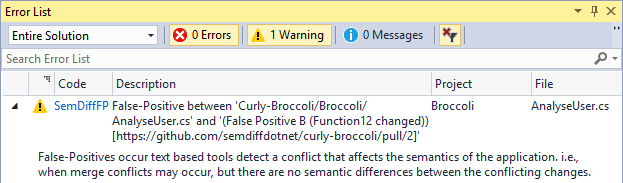
\includegraphics[scale=1]{FalsePositiveErrorList}
\caption{Visual Studio's error list showing a false-positive reported in the 
test repo}
\label{fperrorlist}
\end{figure}

\begin{figure}[!htb]
\centering
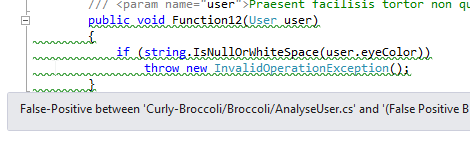
\includegraphics[scale=1]{FalsePositiveHoverOver}
\caption{False positives support warnings with squiggles and hover over 
messages. This shows that the changes to Function12 could cause a 
false-positive}
\label{fphoverover}
\end{figure}

\subsubsection{Future Work}

The false positive warnings display correctly, however there are a few ways 
that they can be improved. Figure~\ref{fphoverover} shows underlines over the 
entire function. With larger functions that will be obnoxious. Instead the 
underline should be be placed under the identifier only. The current message 
format also doesn't specify whether the the current message was moved locally 
or remotely. An improvement would be displaying something like ``method has 
been moved, but was edited in a pull request'' or ``edited method was moved in a 
pull request.''

\newpage

%%%%%%%%%%%%%%%%%%%%%%%%%%%%%%%%%%%%%%%%%%%%%%%%%%%%%%%%%%%%%%%%%%%%%%%%%%%%%%%
\subsection{Displaying False-Negatives Warnings in Error List}%%%%%%%%%%%%%%%%%
%%%%%%%%%%%%%%%%%%%%%%%%%%%%%%%%%%%%%%%%%%%%%%%%%%%%%%%%%%%%%%%%%%%%%%%%%%%%%%%

\textbf{Requirement:}

\begin{quote}

SemDiff will display a warning in the ``Error List'' (at compile time) when a 
false-negative occurs between the semantics of the classes represented by the 
local files and the classes represented by the remote files retrieved from a 
pull request.

SemDiff will show that a false-negative was detected.

SemDiff will show which classes are in conflict.

SemDiff will show the name of the file in conflict.

SemDiff will provide a link to the pull request.

\end{quote}

\subsubsection{Progress}

SemDiff displays false negative warnings as intended. The format of 
warnings is \textit{``False-Negatives for type `$<$Type Name (Base 
Class)$>$' between `($<<$Title of Pull Request$>$)[$<$Link to 
Github$>$]'\,''}. An example of the warning is shown in 
Figure~\ref{fnerrorlist}. That error was collected by cloning the test repo 
and checking out the branch that creates a derived class.

\begin{figure}[!htb]
\centering
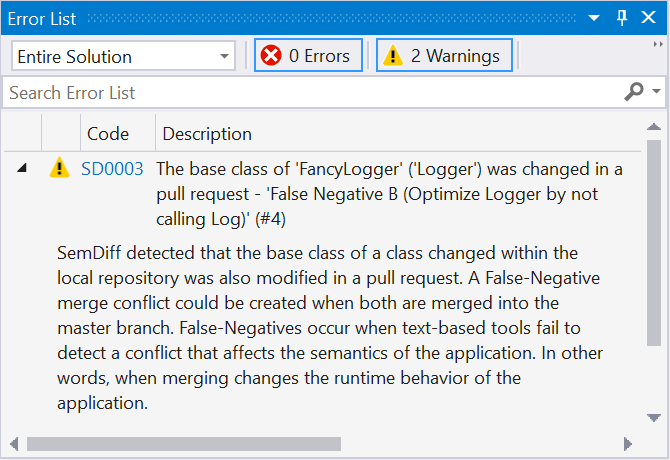
\includegraphics[scale=1]{FalseNegativeErrorList}
\caption{Visual Studio's error list showing two false-negatives reported in 
the test repo}
\label{fnerrorlist}
\end{figure}

\subsubsection{Future Work}

Unlike the false positives messages, false negative messages don't currently 
report a location. This prevents hover over errors from being created. Before 
final release the team will need to decide where to report as the location 
(derived class or base class) and implement the location.

%%%%%%%%%%%%%%%%%%%%%%%%%%%%%%%%%%%%%%%%%%%%%%%%%%%%%%%%%%%%%%%%%%%%%%%%%%%%%%%
\subsection{NuGet Package}%%%%%%%%%%%%%%%%%%%%%%%%%%%%%%%%%%%%%%%%%%%%%%%%%%%%%
%%%%%%%%%%%%%%%%%%%%%%%%%%%%%%%%%%%%%%%%%%%%%%%%%%%%%%%%%%%%%%%%%%%%%%%%%%%%%%%

\textbf{Requirement:}

\begin{quote}

SemDiff will provide a NuGet package that can be installed to a VS project as 
an Analyzer.

\end{quote}

\subsubsection{Progress}
The project currently produces a NuGet package. Figures \ref{pacmansmall} and 
\ref{pacman} shows how the package appears in the NuGet package manager. The 
package is currently available in the NuGet Gallery and can be installed with 
^Install-Package SemDiff -Pre^. The package can also be viewed at 
\url{https://www.nuget.org/packages/SemDiff}. That page contains interesting 
information including the number of times the package has been downloaded.

\begin{figure}[!htb]
\centering
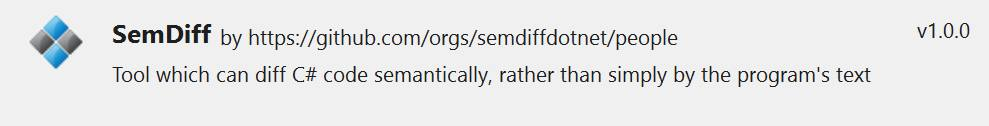
\includegraphics[scale=1]{SemDiffInPackageManagerSmall}
\caption{This is how the SemDiff package is displayed in the NuGet package 
manager}
\label{pacmansmall}
\end{figure}

\begin{figure}[!htb]
\centering
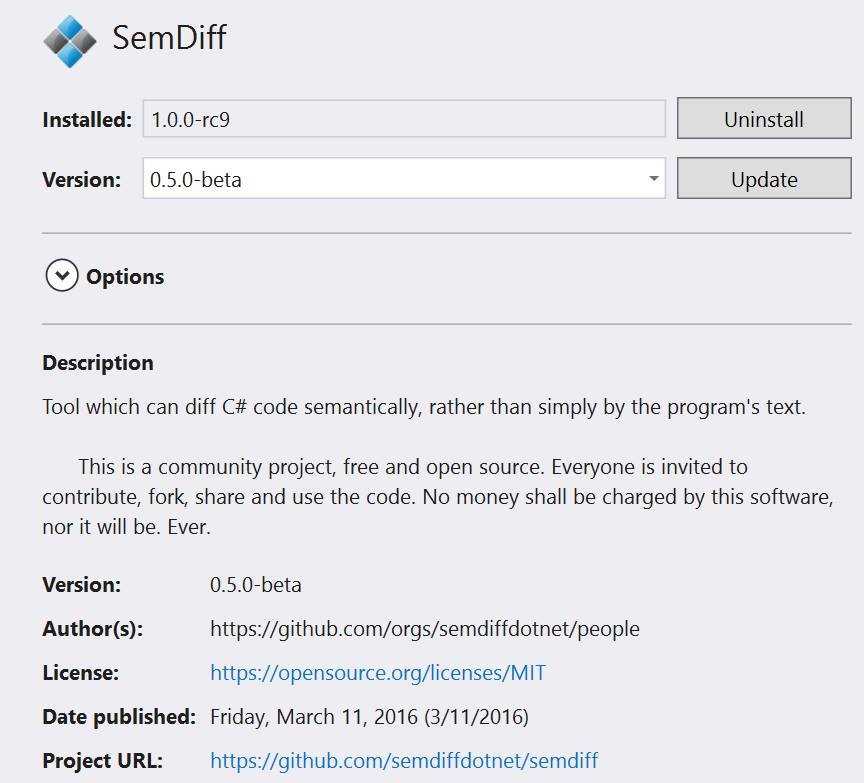
\includegraphics[scale=.8]{SemDiffInPackageManager}
\caption{After the package is selected, this larger window is displayed in the 
NuGet package manager}
\label{pacman}
\end{figure}

\subsubsection{Future Work}

The package could be improved by providing an icon for the package, replacing 
the blue icon with white dots. Additionally, after the package is installed, 
the dependencies show up in the analyzer section of the solution explorer, 
affecting the user experience.

\subsubsection{Problems}

Learning the nuspec configuration format was a significant barrier for this 
requirement. Few people have documented building a NuGet package for Roslyn 
Analyzers. Analyzers are very different from most packages and require a 
different method for building the NuGet package. For example, packages 
usually have dependencies, but analyzers cannot have dependencies because 
that would result in extra packages being installed to the project.

\newpage

%%%%%%%%%%%%%%%%%%%%%%%%%%%%%%%%%%%%%%%%%%%%%%%%%%%%%%%%%%%%%%%%%%%%%%%%%%%%%%%
\subsection{Performance}%%%%%%%%%%%%%%%%%%%%%%%%%%%%%%%%%%%%%%%%%%%%%%%%%%%%%%%
%%%%%%%%%%%%%%%%%%%%%%%%%%%%%%%%%%%%%%%%%%%%%%%%%%%%%%%%%%%%%%%%%%%%%%%%%%%%%%%

\textbf{Requirement:}

\begin{quote}

SemDiff will minimally impact VS performance.

\end{quote}

\subsubsection{Progress}

Async functions were implemented in the request logic to improve the time to 
retrieve data from GitHub, however little performance tuning has been done. 
The table on the SemDiff wiki (on the `Performance' page seen in 
Figure~\ref{wikilist}) will be filled with comparison times for compilation 
with and without SemDiff. 

\subsubsection{Problems}

Initially, the team planned to time the compilation inside of Visual Studio, 
however after more of the project was completed it was discovered that Visual 
Studio actually compiles the solution and then, after compilation is 
complete, it runs any code analysis in the background. Although performance 
of SemDiff is still a high priority, Visual Studio already makes sure that 
analyzers cannot affect performance or compile time. Another side effect of 
this discovery is that SemDiff can no longer time compilation inside of 
Visual Studio because there is no way to determine when it finishes running.
 
There are at least two potential solutions to this problem, but the team has 
not yet determined the best solution. One option is to add code into the 
project that uses the built in ^Stopwatch^ to time how much time SemDiff adds 
to compilation. Another option is to use the Visual Studio command line 
(^devenv.exe^) to compile with and without the SemDiff package installed.

%%%%%%%%%%%%%%%%%%%%%%%%%%%%%%%%%%%%%%%%%%%%%%%%%%%%%%%%%%%%%%%%%%%%%%%%%%%%%%%
\subsection{Informative Alerts}%%%%%%%%%%%%%%%%%%%%%%%%%%%%%%%%%%%%%%%%%%%%%%%%
%%%%%%%%%%%%%%%%%%%%%%%%%%%%%%%%%%%%%%%%%%%%%%%%%%%%%%%%%%%%%%%%%%%%%%%%%%%%%%%

\textbf{Requirement:}

\begin{quote}

Alerts will be informative

\end{quote}

This requirement was added to enhance our specific requirements for 
false-positive and false-negative warnings by emphasizing the importance of 
understandable alerts and making sure the user has a good experience. This is 
extremely important because alerts are the only way that SemDiff communicates 
with the user. Therefore, alerts must contain all the information required to 
understand why an alert was triggered without being cryptic. SemDiff's alerts 
are currently informative, but will continue to evolve.

%%%%%%%%%%%%%%%%%%%%%%%%%%%%%%%%%%%%%%%%%%%%%%%%%%%%%%%%%%%%%%%%%%%%%%%%%%%%%%%
\subsection{GitHub Project Hosting}%%%%%%%%%%%%%%%%%%%%%%%%%%%%%%%%%%%%%%%%%%%%
%%%%%%%%%%%%%%%%%%%%%%%%%%%%%%%%%%%%%%%%%%%%%%%%%%%%%%%%%%%%%%%%%%%%%%%%%%%%%%%

\textbf{Requirement:}

\begin{quote}

All source code, documentation, and issue tracking should be hosted publicly 
on GitHub. The GitHub wiki shall contain documentation for the project 
including a Getting Started guide, an API Guide with code examples, and 
motivational purpose of the project.

\end{quote}

\begin{figure}[!h]
\centering
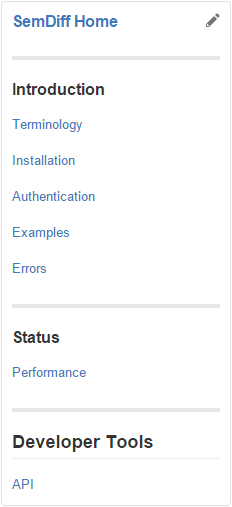
\includegraphics[scale=.9]{WikiList}
\caption{List of all pages captured from the wiki}
\label{wikilist}
\end{figure}

\subsubsection{Progress}
The project source code is hosted on GitHub, and the team has also used the 
issue tracking, pull requests, and milestone features built into GitHub. 
Currently there are 4 milestones, 8 open issues, 18 closed issues, and 28 
closed pull requests. The wiki is setup, but many pages remain incomplete. 
Figure~\ref{wikilist} shows the pages that are currently created.

\subsubsection{Future Work}

To complete this requirement, a lot more content needs to be added to the 
wiki, including an API Guide and code examples that detail the parts of the 
application. The Getting Started Guide will need to be filled with simple yet 
important information. A performance section that details how SemDiff affects 
the speed of compilation requires tests to be run and that information must 
be added to the page. In the future there will be an API Guide using the XML 
documentation inside of the source code.

\subsubsection{Problems}

The team had some difficulty in week one and two with Shawn not being able to 
commit to GitHub or make new issues, however that was resolved before it 
impacted productivity. There was also had some difficulty with using Git. The 
Git plugin for Visual Studio has some usability problems. This led to some 
code being pushed directly to the master branch. To resolve the issue (and 
submit the pull request with peer review), the team had to learn how to 
revert commits and revert merge commits. Before things were figured out a 
long string of revert commits were left behind. Since the problem was 
resolved, things have worked more smoothly.

%%%%%%%%%%%%%%%%%%%%%%%%%%%%%%%%%%%%%%%%%%%%%%%%%%%%%%%%%%%%%%%%%%%%%%%%%%%%%%%
\subsection{MIT Licensing}%%%%%%%%%%%%%%%%%%%%%%%%%%%%%%%%%%%%%%%%%%%%%%%%%%%%%
%%%%%%%%%%%%%%%%%%%%%%%%%%%%%%%%%%%%%%%%%%%%%%%%%%%%%%%%%%%%%%%%%%%%%%%%%%%%%%%

\textbf{Requirement:}

\begin{quote}

All outputs of the project should be open source and licensed with the MIT 
license.

\end{quote}

A copy of the MIT license is available at the root of the GitHub repo and the 
final package includes a link to the MIT license. In the future, a comment 
will be added to the top each file. This is not strictly required by the MIT 
license (unlike the GPLv3), but is still considered a best practice. The line 
that will be added is shown in Figure~\ref{mitheader}. That line was inspired 
by a similar line that appears in the Roslyn source code.

\begin{figure}[!htb]
\centering
\begin{lstlisting}
// Copyright (c) 2015 semdiffdotnet. Distributed under the MIT License. 
// See LICENSE file or opensource.org/licenses/MIT.
\end{lstlisting}
\caption{License Preamble that will be added to the top of all developer 
produced code}
\label{mitheader}
\end{figure}

%%%%%%%%%%%%%%%%%%%%%%%%%%%%%%%%%%%%%%%%%%%%%%%%%%%%%%%%%%%%%%%%%%%%%%%%%%%%%%%
\subsection{Documentation in Code}%%%%%%%%%%%%%%%%%%%%%%%%%%%%%%%%%%%%%%%%%%%%%
%%%%%%%%%%%%%%%%%%%%%%%%%%%%%%%%%%%%%%%%%%%%%%%%%%%%%%%%%%%%%%%%%%%%%%%%%%%%%%%

\textbf{Requirement:}

\begin{quote}

Source code will contain header comments on public classes, public 
interfaces, and public methods. Methods will only contain comments that help 
explain the function of obscure code.

\end{quote}

The public items have good descriptions using the XML documentation, and 
there are no redundant comments inside the methods. Any methods added in the 
future will also have full XML comments.

%%%%%%%%%%%%%%%%%%%%%%%%%%%%%%%%%%%%%%%%%%%%%%%%%%%%%%%%%%%%%%%%%%%%%%%%%%%%%%%
\subsection{Development Technology}%%%%%%%%%%%%%%%%%%%%%%%%%%%%%%%%%%%%%%%%%%%%
%%%%%%%%%%%%%%%%%%%%%%%%%%%%%%%%%%%%%%%%%%%%%%%%%%%%%%%%%%%%%%%%%%%%%%%%%%%%%%%

\textbf{Requirement:}

\begin{quote}

SemDiff will be built using C\# and the Roslyn API.

\end{quote}

SemDiff is implemented in C\# and uses the Roslyn APIs to compare syntax 
trees. This project would not have been possible without Rosyln. A 
black box compiler would have nessenitated writing a parser and semantic 
analyzer to complete the project. Roslyn is used in multiple places in SemDiff, 
the most interesting uses of Roslyn is the ^ForFalseNegative^ function, shown 
in Figure~\ref{anforfn}, that uses the ^SemanticModel^ to find the base class 
of the current file.

%-----------------------------------------------------------------------------|
%%%%%%%%%%%%%%%%%%%%%%%%%%%%%%%%%%%%%%%%%%%%%%%%%%%%%%%%%%%%%%%%%%%%%%%%%%%%%%|
\section{Conclusion}%%%%%%%%%%%%%%%%%%%%%%%%%%%%%%%%%%%%%%%%%%%%%%%%%%%%%%%%%%|
%%%%%%%%%%%%%%%%%%%%%%%%%%%%%%%%%%%%%%%%%%%%%%%%%%%%%%%%%%%%%%%%%%%%%%%%%%%%%%|
%-----------------------------------------------------------------------------|

From the above information, it is clear that SemDiff is a beta level project. 
There is a significant amount of testing and documentation for next term, but 
the project will be ready and satisfy the requirements by Expo.

%-----------------------------------------------------------------------------|
%%%%%%%%%%%%%%%%%%%%%%%%%%%%%%%%%%%%%%%%%%%%%%%%%%%%%%%%%%%%%%%%%%%%%%%%%%%%%%|
\section{Glossary}%%%%%%%%%%%%%%%%%%%%%%%%%%%%%%%%%%%%%%%%%%%%%%%%%%%%%%%%%%%%|
%%%%%%%%%%%%%%%%%%%%%%%%%%%%%%%%%%%%%%%%%%%%%%%%%%%%%%%%%%%%%%%%%%%%%%%%%%%%%%|
%-----------------------------------------------------------------------------|

                                   %The label width should be the longest term
\begin{description}[\IEEEsetlabelwidth{False-Positive:}\IEEEusemathlabelsep] 

\item[.NET:] Framework that provides the runtime and core libraries for C\# 
and other languages.

\item[API:] An Application Programming Interface represents the point of 
interaction between a system and other systems that utilize it.

\item[AST:] An Abstract Syntax Tree is a parsed data structure that represents 
all of the tokens in source code.

\item[Code Smell:] Indicators found in source code that indicate deeper 
problems in the system.

\item[C\#:] The C\# 6.0 general purpose programming language.

\item[Diff:] Tool that compares two versions of code to look for changes.

\item[False-Positive:] A condition where text-based tools  detect a conflict 
but according the code's semantics there should be no conflict. The `moved 
method' situation exemplifies a common false-positive condition.

\item[False-Negative:] A condition that occurs when text-based tools do not 
find a conflict between changed files even though there is a conflict 
according to the code's semantics. The `Logger' situation exemplifies a 
false-negative condition.

\item[GitHub:] Project hosting website that provide version control, issue 
tracking, and documentation tools for software projects.

\item[IDE:] An Integrated Development Environment is a text editor that 
provides tools like debuggers, compilers, code completion, and refactoring 
tools to improve developer productivity.

\item[KISS:] A software enginering principle and an acronym that stands for 
`keep it short and simple;' the idea of KISS is to make things `as simple as 
possible, no simpiler'.

\item[NuGet Package:] Open-source package manager for the Microsoft 
development platform that provides the ability to produce and consume package 
in Visual Studio.

\item[Roslyn:] Open-source C\# and Visual Basic compiler with a rich code 
analysis API. Roslyn enables building code analysis tools with the same API 
Visual Studio uses.

\item[Semantics:] Executing behavior of a program and the meaning/purpose of 
what is being executed. 

\item[VS:] Visual Studio 2015 is a popular IDE for working with C\#.

\end{description}

\end{document}
